% Appendix A

\chapter{Details on the Bubble Growth Calculation}

%----------------------------------------------------------------------------------------

To further study the bubble growth process, we will try to derive an analytic

In this section, computations are conducted using the spherical coordinates $\left(\vect{e_{r}}, \vect{e_{\theta}}, \vect{e_{\varphi}}\right)$ with coordinates $(r, \theta, \phi)$. 

\begin{figure}[h!]
\centering
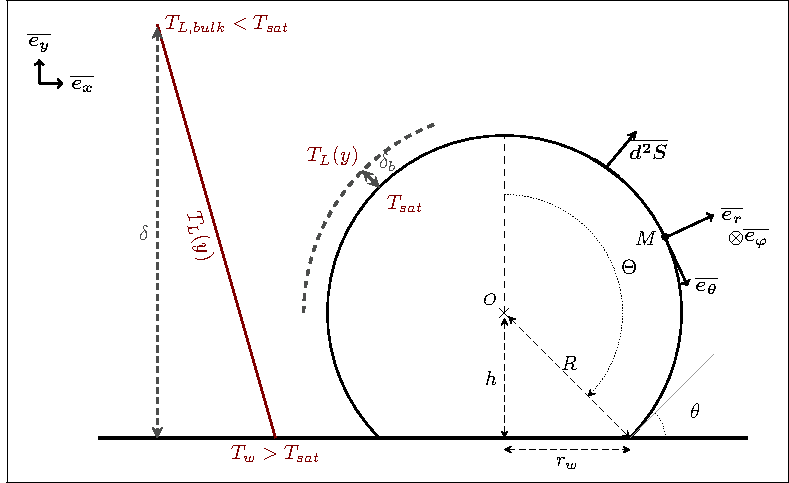
\includegraphics[width=0.7\linewidth]{img/growth/growth_analytical.pdf}
\caption{Studied geometry}
\label{fig:anal_growth}
\end{figure}

\npar
Geometrical definitions :
\begin{itemize}
\item $\Theta=\pi - \theta$ the angular portion of the truncated sphere in spherical coordinates ;
\item $r_{w}=R\sin{\theta}=-R\sin{\Theta}$ the bubble foot radius ;
\item $h=R\cos{\theta}=-R\cos{\Theta}$ the distance between the wall and the center of the bubble ($>0$ if $\theta < \pi/2$, $<0$ otherwise) ;
\item $R$ and $V=\frac{4}{3}\pi R^{3} f_{V}\left(\theta\right)$ the radius and the volume of the bubble ;
\item $\vect{d^{2}S}=R^{2}\sin{\theta}\dtheta d\varphi \vect{e_{r}}$ the surface vector in spherical coordinates ;
\item $y=R\cos{\theta}+h = R\left(\cos{\theta} - \cos{\Theta}\right)$ the distance to the wall in cartesian coordinates.
\end{itemize}


\npar
Thermal-hydraulics definitions :
\begin{itemize}
\item $\Delta T_{L} = T_{sat}-T_{\infty}$ et $\Delta T_{w}=T_{w}-T_{sat}$ the subcooling of the liquid and the wall superheat respectively ;
\item $\delta$ et $\delta_{b}$ the flow boundary layer thickness and the bubble boundary layer thickness respectively ;
\item $d^{2} Q_{b}$ the heat received by the bubble between $t$ and $t+dt$ through the surface $d^{2}S$ ;
\item $\lambda$, $\rho$, $c_{p}$, $\eta$, $h$ the thermal conductivity, density, heat capacity, thermal diffusivity and mass enthalpy respectively ($l$ standing for liquid  and $g$ for gas) ;
\item $\text{Ja}_{w}=\Delta T_{w} \rho_{L}c_{p,L}/(h_{LV}\rho_{V})$ the wall superheat (or boiling) Jakob number and $\text{Ja}_{L}=\Delta T_{L} \rho_{L}c_{p,L}/(h_{LV}\rho_{V})$ the subcooled liquid (or condensation) one.
\end{itemize}

\npar


The thermal boundary layer of the flow is assumed to follow a linear profile, giving the the expression :

\begin{align}
T_{l}\left(y\right)=T_{w}+\frac{T_{\infty}-T_{w}}{\delta} y
\end{align}


If we consider that the bubble stays at a temperature close to $T_{sat}$, the radial component of the temperature gradient at the bubble's interface yields :

\begin{align}
\grad{T} \cdot \vect{er} = \dpartial{T}{r}\left(R, \theta, \phi\right)\approx\frac{T_{\l}(y)-T_{sat}}{\delta_{b}}
\end{align}

\npar



Applying Fourier's law to the liquid close to the bubble : $\vect{j_{Q}}=-\lambda_{l} \grad{T}$, then the bubble receives between $t$ and $t+dt$ through $d^{2}S$ :

\begin{align}
d^{2}Q_{b}&=\vect{j_{Q}} \cdot \left(-\vect{d^{2}S}\right)\\
&=\lambda_{l} \dpartial{T}{r}\left(R,\theta, \varphi\right) R^{2}\sin{\theta} d\theta d\varphi\\
&\approx\lambda_{l} \frac{T_{l}\left(y\right)-T_{sat}}{\delta_{b}}R^{2}\sin{\theta}d\theta d\varphi\\
&=\lambda_{l} \frac{1}{\delta_{b}}\left[T_{w}+\frac{T_{\infty}-T_{w}}{\delta}y - T_{sat}\right]R^{2}\sin{\theta}d\theta d\varphi\\
&=\frac{\lambda_{l}}{\delta_{b}}\left[\Delta T_{w}-\frac{\Delta T_{w} + \Delta T_{l}}{\delta}R\left[\cos{\theta} - \cos{\Theta}\right]\right]R^{2}\sin{\theta}d\theta d\varphi\\
&=\frac{\lambda_{l}}{\delta_{b}}\left[\Delta T_{w}R^{2}\sin{\theta}-\frac{\Delta T_{w}+\Delta T_{l}}{\delta}R^{3}\left[\cos{\theta}-\cos{\Theta}\right]\sin{\theta}\right] d\theta d\varphi
\end{align}

\npar
The total heat flux received by the bubble can then be derived, supposing that $\delta_{b}$ is constant all around the bubble between $t$ and $t+dt$ :

\begin{align}
Q_{b}&=\int_{\varphi=0}^{\varphi=2\pi} \int_{\theta=0}^{\Theta}{d^{2}Q_{b}}\\
&= \frac{2\pi \lambda_{l}}{\delta_{b}}\left[\int_{0}^{\Theta} \Delta T_{w} R^{2} \sin{\theta}d\theta + \int_{0}^{\Theta} \frac{\Delta T_{w} + \Delta T_{l}}{\delta} R^{3} \cos{\Theta}\sin{\theta}d\theta - \int_{0}^{\Theta} \frac{\Delta T_{w} + \Delta T_{l}}{\delta} R^{3} \cos{\theta}\sin{\theta}d\theta\right]\\
&=\frac{2\pi \lambda_{l}}{\delta_{b}} \left[\Delta T_{w} R^{2} \left(1-\cos{\Theta}\right) + \frac{\Delta T_{w} + \Delta T_{l}}{\delta}R^{3}\left[\cos{\Theta}\left(1-\cos{\Theta}\right)- \frac{1}{4}\left(1 - \cos{2\Theta}\right)\right]\right]\\
&=\frac{2\pi \lambda_{l} R^{2}}{\delta_{b}}\left[\frac{-R}{2\delta}\left(\Delta T_{w} + \Delta T_{l}\right)\left(1 + 2\cos{\alpha} + \cossq{\alpha}\right) + \Delta T_{w} \left(1 + \cos{\alpha } \right) \right]\\
&=\frac{2\pi \lambda_{l} R^{2}}{\delta_{b}}\left(1+\cos{\alpha}\right)\left[\Delta T_{w} - \frac{R}{2\delta}\left(\Delta T_{w} + \Delta T_{l}\right) \left(1 + \cos {\alpha} \right )\right]
\end{align}


\npar
Between $t$ and $t+dt$, the bubble receives a $Q_{b}dt$ energy amount through thermal diffusion. Assuming this energy solely contributes to evaporation of the surrounding liquid, the resulting mass of generated vapor is :

\begin{align}
&dm_{g} = \rho_{g} dV = \frac{Q_{b}dt}{h_{lg}}\\
\text{then } &\frac{dV}{dt}=\frac{Q_{b}}{\rho_{g}h_{lg}}
\end{align}

Since $V=\frac{4}{3}\pi R^{3} f_{V}\left(\alpha\right)$, we can write : 

\begin{align}
\frac{dV}{dt}=\frac{4}{3}\pi f_{V}\left(\alpha\right) 3R^{2}\frac{dR}{dt}
\end{align}

Then :

\begin{align}
\frac{dR}{dt}&=\frac{1}{4\pi R^{2}f_{V}\left(\alpha\right)} \frac{1}{\rho_{g} h_{lg}} \frac{2 \pi \lambda_{l} R^{2}}{\delta_{b}}\left(1+\cos{\alpha}\right)\left[\Delta T_{w} - \frac{R}{2\delta}\left(\Delta T_{w} + \Delta T_{l}\right) \left(1 + \cos{\alpha} \right )\right]\\
&= \frac{1}{2f_{V}\left(\alpha\right)}\frac{\Delta T_{w}}{h_{lg}\rho_{g}}\frac{\lambda_{l}}{\delta_{b}}\left(1+\cos{\alpha}\right)\left[1 - \frac{R}{2\delta}\left(1 + \frac{\Delta T_{l}}{\Delta T_{w}}\right) \left(1 + \cos {\alpha} \right )\right]\\
&=\frac{\text{Ja}_{w} \eta_{l}}{2 \delta_{b} f_{V}\left(\alpha\right)}\left(1+\cos{\alpha}\right)\left[1 - \frac{R}{2\delta}\left(1 + \frac{\text{Ja}_{l}}{\text{Ja}_{w}}\right) \left(1 + \cos{\alpha} \right )\right]
\end{align}

If we define :

\begin{align}
a = \frac{\text{Ja}_{w}\eta_{l}}{4 \delta_{b} \delta f_{V} \left(\alpha\right)} \left(1 + \frac{\text{Ja}_{l}}{\text{Ja}_{w}}\right) \left(1 + \cos{\alpha}\right)^{2} \text{ et } b = \frac{\text{Ja}_{w}\eta_{l}}{2 \delta_{b} f_{V}\left(\alpha\right)}\left(1 + \cos{\alpha}\right)
\end{align}

Finally : 

\begin{align}
\frac{dR}{dt} + aR = b
\end{align}


\npar

Solutions of this differential equation depend on the hypothesis over $\delta$ and $\delta_{b}$. In a first approach, we will consider that $\delta$ does not vary during the whole bubble growth. This thickness could be expressed using boundary layer thickness correlations for example (laminar or turbulent depending on the Reynolds number). 

\npar

On the other hand, we will consider 3 different choices to model $\delta_{b}$ :


\npar
\subsection{Case 1 : $\delta_{b}$ is constant}


This is a \textbf{strong assumption} since it means that $\delta_{b}$ does not depend on the temperature and the flow shear rate facing the bubble. In this case, $a$ and be are constant, giving : 


\begin{align}
\frac{dR}{dt} + aR = b
\end{align}


With the initial condition $R(t=0)=0$ the solution of this differential equation is : 

\begin{align}
R\left(t\right)=\frac{b}{a}\left(1 - e^{-at}\right) \text{ where } \frac{b}{a} = \frac{2\delta}{\left(1 + \frac{\text{Ja}_{l}}{\text{Ja}_{w}}\right)\left(1 + \cos{\alpha} \right )}=R_{\infty} \text{ is the final bubble equilibrium radius.}
\end{align}


\subsection{Case 2 : $\delta_{b}=\sqrt{\eta_{l}t}$}
\npar

This expression derives from the growth of a boundary layer through pure diffusion, as studied by \textsc{Legendre} \etal

Such a boundary layer thickness is also used when one writes the quenching heat flux (see Section \ref{sec:model} and \textsc{Del Valle \& Kenning} work).

In this case, this means that the boundary layer around the bubble interface grows through diffusion only.

\npar

Thus, it yields :

\begin{align}
\frac{dR}{dt}\parth{t}+a\parth{t}R\parth{t}=b\parth{t}
\end{align}

\begin{align}
\label{eq:coeff_expgrowth}
a(t)=\frac{\Ja_{w}\sqrt{\eta_{l}}}{4\delta f_{V}\parth{\alpha}\sqrt{t}}\parth{1+\frac{\Ja_{l}}{\Ja_{w}}}\parth{1+\cos{\alpha}}^{2}=K_{a}t^{-1/2} \text{ and } b(t)=\frac{\Ja_{w}\sqrt{\eta_{l}}}{2f_{V}\parth{\alpha}\sqrt{t}}\parth{1+\cos{\alpha}}=K_ {b}t^{-1/2}
\end{align}

With the initial condition $R\parth{t=0}=0$, the solution is given by : 

\begin{align}
R\parth{t}=R_{\infty}\parth{1-e^{-2K_{a}\sqrt{t}}} \text{ avec } R_{\infty}=\frac{K_{b}}{K_{a}}
\end{align}

\npar
\subsection{Case 3 : $\delta_{b}=CR$}
\npar

In this last case, the bubble boundary layer is assumed to by proportional to the bubble radius $R$, through a constant coefficient $C$. This yields :


\begin{align}
a(t)=\frac{\Ja_{w}\eta_{l}}{4\delta f_{V}\parth{\alpha}CR\parth{t}}\parth{1+\frac{\Ja_{l}}{\Ja_{w}}}\parth{1+\cos{\alpha}}^{2}=K'_{a}\frac{1}{R\parth{t}} \text{ et } b(t)=\frac{\Ja_{w}\eta_{l}}{2f_{V}\parth{\alpha}CR\parth{t}}\parth{1+\cos{\alpha}}=K'_ {b}\frac{1}{R\parth{t}}
\end{align}

Giving :

\begin{align}
&\frac{dR}{dt}\parth{t} + K'_{a} = K'_{b}\frac{1}{R\parth{t}}
\end{align}

Which the solution with the initial condition $R\parth{t=0}=0$ is :

\begin{align}
R\parth{t}=R_{\infty}\parth{ \text{W}\parth{-e^{-t{K'_{a}}^{2}/K'_{b}-1} } +1}
\end{align}

With $\text{W}$ being the \textsc{Lambert} function defined as the reciprocal function of $w \rightarrow we^{w}$ on $\mathbb{C}$.
